\documentclass[11pt,letterpaper,titlepage]{article}
\usepackage{amssymb,amsmath}
\usepackage{graphicx}
\usepackage{subfig} % For subfigures
\usepackage{array}
\usepackage{colortbl}
\usepackage{tikz} % For awesome graphics diagrams
\usepackage{float}
\usepackage{fancyhdr} % For header
\usepackage[left=1in,top=1in,right=1in,bottom=1in]{geometry}
\parskip 7.2pt
%\parindent 0pt

\newcommand{\note}[1]{\textbf{NOTE: #1}}

\setlength{\headheight}{15.2pt}
\pagestyle{fancy}
\lhead{} \chead{} \rhead{ ECE 739 Project, Winter 2011} \lfoot{From: P. Chrapka, M. R Wirtzfeld} \cfoot{To:  Dr. S. Haykin} \rfoot{\thepage} \renewcommand{\headrulewidth}{0.4pt} \renewcommand{\footrulewidth}{0.4pt}

\numberwithin{equation}{section}
\numberwithin{figure}{section}
\numberwithin{table}{section}

\begin{document}

\title{ECE 739 - Neural Networks\\Computer Experiment:\\SVM vs EKF-trained MLP}
\author{Philip Chrapka}
\date{August 26, 2011}
\maketitle

\tableofcontents
\clearpage

\section{Introduction}

As more difficult problems are encountered in research, more complex algorithms are required to help solve them. Basic statistical analysis is typically not enough to differentiate between different classes of data points, especially when the data is not linearly separable. This is where neural networks and learning machines contribute most. These algorithms are designed in such a manner that they can adapt and learn from the data that is provided. The question that remains is which provides better performance with the least amount of computational time.

\section{Concepts}
\label{sec:concepts}

\subsection{Support Vector Machines (SVM)}

The support vector machine (SVM) is based on determining an optimal hyperplane to separate two classes within the same data set. By using a suitable data set we can train the SVM to distinguish between these two classes. The training data can be defined as follows
\begin{gather}
  \mathcal{T} = \left\{ \mathbf{x}_i, d_i \right\}_{i=1}^{N}
\end{gather}
where \(\mathbf{x}_i\) represents the \textit{i}th sample and \(d_i\) represents the desired output for the \textit{i}th sample.

The hyperplane can be defined by the following equation
\begin{gather}
	\label{eq:hyperplane}
	\mathbf{w}^T\mathbf{x} + b = 0
\end{gather}
where \(\mathbf{w}\) represents a weight vector and \(b\) represents a bias.

For separable data following Equation~\ref{eq:3} below, the support vector machine attempts to construct the hyperplane such that the margin of separation is maximized. That is, it attempts to maximize the distance between the closest points to the hyperplane and the hyperplane itself.
\begin{gather}
  \label{eq:3}
  d_i\left( \mathbf{w}^T\mathbf{x}_i + b\right) \geq 1, \quad i=1,2,...,N
\end{gather}

In the case of non-separable data, data points will inevitably fall within the margin of separation or even on the other side of the hyperplane. As a result, slack variables, \(\xi\), are introduced that account for the difference between a point's current position and its ideal position. The equation describing the hyperplane becomes
\begin{gather}
  \label{eq:4}
  d_i\left( \mathbf{w}^T\mathbf{x}_i + b\right) \geq 1-\xi_i, \quad i=1,2,...,N
\end{gather}
To determine the optimal hyperplane we want to minimize the classification error rate, which can be approximated by minimizing the cost function \(\phi(\xi)\),
\begin{gather}
  \label{eq:5}
  \phi(\xi) = \sum_{i=1}^{N} \xi_i
\end{gather}
which in turn can be further simplified to
\begin{gather}
  \label{eq:6}
  \phi(\mathbf{w},\xi) = \frac{1}{2}\mathbf{w}^T\mathbf{w} + C \sum_{i=1}^{N} \xi_i
\end{gather}
where the optimization is performed with respect to the weight vector, \(\mathbf{w}\). The C parameter corresponds to the complexity of the SVM and describes the quality of the data \cite{Haykin2008}. A larger C parameter indicates that the training data is of higher quality and contains little noise. In this way the SVM can have a decision surface that is more sensitive to the input data.

The optimization can be performed using the method of Lagrange multipliers. For a more complete treatment of this optimization problem, we refer the reader to \cite{Haykin2008}.

\subsection{Multilayer Perceptron (MLP)}
\label{sec:mult-perc}

Multilayer perceptrons (MLPs) are networks modeled on the basic concept of the biological neuron found in neural tissue. Figure~\ref{fig:neuron} shows how a single neuron can be transformed into a computational model. Each node has a variable number of inputs \(x_m(n)\). In turn, each of these inputs are weighted differently according to the desired input-output characteristics of the neuron. These weights are represented by \(w_{ji}\). Each node can also have a constant input which is also known as a bias, \(b\).

\tikzstyle{node} = [circle, draw, thick, minimum size=4pt, inner sep=0pt]
\begin{figure}[!ht]
\centering
\begin{tikzpicture}[]
	\node [node,label={left:\(x_0 = 1\)}]		(x0)     	at (1,3) {};
	\node [node,label={left:\(x_1(n)\)}]   	 	(x1)     	at (1,2) {};
	\node      						(dots1) 	at (1,1) {\(\vdots\)};
	\node [node,label={left:\(x_i(n)\)}]    		(xi) 		at (1,0) {};
	\node 					    		(dots2) 	at (1,-1) {\(\vdots\)};
	\node [node,label={left:\(x_m(n)\)}] 		(xm) 		at (1,-2) {};
	
	\node [node,label={above:\(v_j(n)\)}] 	(vj) 		at (4,0) {};
	
	\node [node,label={above:\(y_j(n)\)}] 		(yj) 		at (6,0) {};
	
	\path[->]
		(x0) 		edge 	node [label={right:\(w_{j0} = b_j(n)\)}] {}	(vj)
		(x1) 		edge 								(vj)
		(xi) 		edge 	node [label={above:\(w_{ji}(n)\)}] {}		(vj)
		(xm)		edge 								(vj)
		
		(vj)		edge 	node [label={above:\(\varphi(\cdot)\)}] {}	(yj)
		;
\end{tikzpicture}
\caption{Flow graph showing a single neuron (Reproduced from \cite{Haykin2008})}
\label{fig:neuron}
\end{figure}

Once the weighted inputs reach the neuron, they are summed and passed through an activation function, \(\varphi\), that produces the final output. This is summarized in Equation \eqref{eq:8}.
\begin{gather}
	\label{eq:8}
	y_j(n) = \varphi \left( \sum_{i=0}^m w_{ji}(n)x_i(n)\right)
\end{gather}

A MLP is essentially a network of individual neurons and can take many forms. The greatest flexibility is offered in the number of hidden layers and the number of nodes within each layer. Figure~\ref{fig:mlp_network} shows an MLP network containing 2 hidden layers and a single output node. It demonstrates how an MLP can have any number of input nodes as well hidden nodes.

\tikzstyle{input} = [rectangle,draw,minimum width=4pt,minimum height=4pt, inner sep=0pt]
\tikzstyle{node_big} = [circle, draw, thick, minimum size=12pt, inner sep=0pt]

\begin{figure}[!ht]
\centering
\begin{tikzpicture}
	% Input layer
	\node [input,label={left:\(x_1(n)\)}]	(x1) 		at (1,5) {};
	\node [input,label={left:\(x_2(n)\)}]	(x2) 		at (1,3) {};
	\node 						(dots1) 	at (1,1) {\(\vdots\)};
	\node [input,label={left:\(x_I(n)\)}]	(x3) 		at (1,0) {};
	% Label
	\node	[text width=1.5cm]			(label1)	at (1,-3) {Input Layer};
	
	% Hidden Layer 1
	% Nodes
	\node [node_big]		(n1_1)	at (3,5) {};
	\node [node_big]		(n1_2)	at (3,3) {};
	\node				(n1_3)	at (3,1) {\(\vdots\)};
	\node [node_big]		(n1_4)	at (3,0) {};
	% Bias nodes
	\node [input,label={below:\(b_{1,1}\)}]	(b1_1)	at (3,4){};
	\node [input,label={below:\(b_{1,2}\)}]	(b1_2)	at (3,2){};
	\node [input,label={below:\(b_{1,J}\)}]	(b1_4)	at (3,-1){};
	% Label
	\node	[text width=1.5cm] 	(label2) 	at (3,-3) {Hidden Layer 1};
	
	% Hidden Layer 2
	% Nodes
	\node [node_big]		(n2_1)	at (5,5) {};
	\node [node_big]		(n2_2)	at (5,3) {};
	\node				(n2_3)	at (5,1) {\(\vdots\)};
	\node [node_big]		(n2_4)	at (5,0) {};
	% Bias nodes
	\node [input,label={below:\(b_{2,1}\)}]		(b2_1)	at (5,4){};
	\node [input,label={below:\(b_{2,2}\)}]		(b2_2)	at (5,2){};
	\node [input,label={below:\(b_{2,K}\)}]		(b2_4)	at (5,-1){};
	%Label
	\node	[text width=1.5cm] 	(label3) 	at (5,-3) {Hidden Layer 2};
	
	
	% Output layer
	\node [node_big,label={right:\(y(n)\)}]	(n3_1)	at (7,3) {};
	\node	[text width=1.5cm]			(label4) 	at (7,-3) {Output Layer};
	
	% Connections
	\foreach \x in {1,...,3}
		\foreach \y in {1,2,4}
		{
			\path[->] (x\x) edge (n1_\y);
		}
		
	\foreach \x in {1,2,4}
		\foreach \y in {1,2,4}
		{
			\path[->] (n1_\x) edge (n2_\y);
		}
		
	\foreach \x in {1,2,4}
		{
			\path[->] (n2_\x) edge (n3_1);
		}
		
	\foreach \x in {1,2,4}
		{
			\path[->] (b1_\x) edge (n1_\x);
		}
		
	\foreach \x in {1,2,4}
		{
			\path[->] (b2_\x) edge (n2_\x);
		}
	
\end{tikzpicture}
\caption{Multilayer Perceptron Network with 2 Hidden Layers}
\label{fig:mlp_network}
\end{figure}


\subsection{Extended Kalman Filter (EKF)}

Kalman filters have numerous applications in technology. In general, Kalman filters have the ability to estimate the state of a process using observations. The state of all processes encountered in the real world are hidden; the exact state is never known. However, we can make measurements that in one way or another describe the state and we can typically propose a model that approximates the process. Kalman filters use this knowledge to calculate an approximation of the state and are very successful in doing so. The basic Kalman filter is based on a linear model. The extended version of the filter includes linear approximations of non-linear models and is appropriately named the extended Kalman filter (EKF). 

The EKF is represented by two equations, the process equation and the measurement equation, which form the state space model. It can be described as follows
\begin{gather}
  \label{eq:7a}
  \mathbf{x}_{k+1} = \mathbf{f}(k, \mathbf{x}_k) + \mathbf{w}_k
\end{gather}
\begin{gather}
  \label{eq:7b}
  \mathbf{y}_k = \mathbf{h}(k, \mathbf{x}_k) + \mathbf{v}_k
\end{gather}
where \(\mathbf{x}_k\) represents the state at time k and \(\mathbf{y}_k\) represents the measurement at time k \cite{Haykin2001}. Equation~\ref{eq:7a} is the process equation which describes the evolution of the state and \(\mathbf{f}\) describes our model of the process. Equation~\ref{eq:7b} is the measurement equation which describes our measurement of the process. Both equations naturally contain noise, represented by \(\mathbf{w}_k\) and \(\mathbf{v}_k\), which is assumed to be independent, zero-mean and Gaussian. The noise processes are also associated with covariance matrices \(\mathbf{Q}_k\) and \(\mathbf{R}_k\), respectively.

The EKF is an iterative algorithm where you can incrementally update the algorithm with new data as it becomes available. The algorithm is described by the following equations which have been reproduced here from \cite{Haykin2001}.

\noindent 
\textit{State estimate propagation}
\begin{gather*}
  \mathbf{\hat{x}}_k^{-} = \mathbf{f}(k,\mathbf{\hat{x}}_{k-1})
\end{gather*}
\textit{Error covariance propagation}
\begin{gather*}
  \mathbf{P}_k^{-} = \mathbf{F}_{k,k-1} \mathbf{P}_{k-1} \mathbf{F}^{T}_{k,k-1} + \mathbf{Q}_{k-1}
\end{gather*}
\textit{Kalman gain matrix}
\begin{gather*}
  \mathbf{G}_k = \mathbf{P}_k^{-} \mathbf{H}_k^T \left[ \mathbf{H}_k \mathbf{P}_k^- \mathbf{H}_k^T + \mathbf{R}_k \right]^{-1}
\end{gather*}
\textit{State estimate update}
\begin{gather*}
  \mathbf{\hat{x}}_k = \mathbf{\hat{x}}_k^- + \mathbf{G}_k \mathbf{y}_k - \mathbf{h}(k,\mathbf{\hat{x}}_k^-)
\end{gather*}
\textit{Error covariance update}
\begin{gather*}
  \mathbf{P}_k = (\mathbf{I} - \mathbf{G}_k \mathbf{H}_k) \mathbf{P}_k^-
\end{gather*}

where
\begin{gather*}
  \mathbf{F}_{k+1,k} = \left. \frac{\partial \mathbf{f}(k,\mathbf{x})}{\partial \mathbf{x}} \right\rvert_{\mathbf{x = \mathbf{x}_k}} \\
  \mathbf{H}_{k} = \left. \frac{\partial \mathbf{h}(k,\mathbf{x})}{\partial \mathbf{x}} \right\rvert_{\mathbf{x = \mathbf{x}_k^-}}
\end{gather*}

The EKF is fairly straightforward to put into practical use however it does have a few complications. The EKF uses a first order Taylor series expansion to approximate the nonlinearity in the process, thus the process should not exhibit significant non-linear characteristics beyond a first-order. In addition, the algorithm requires the computation of Jacobians which can be a practical limitation.

\subsection{EKF-trained MLP}
\label{sec:ekf-trained-mlp}

At first it may not be obvious, but training a MLP neural network is a perfect application for the EKF algorithm. The main idea behind training a neural network is determining an optimal set of weights that can perform the required classification task. If the problem is formulated in such a way that the set of weights in the MLP describe the state of the process, then we can easily apply the EKF. The various parameters of the EKF algorithm are described in the context of training an MLP network in Table~\ref{table:ekf_parameters}.

\begin{table}[ht]
  \centering
  \begin{tabular}{ c l }
    \rowcolor[gray]{0.8}
    \textbf{Parameter} & \textbf{Description} \\
    \(\mathbf{x}\) & Weight vector \\
    \(\mathbf{f}\) & Nonlinear model to describe weight vector training process \\
    \(\mathbf{w}\) & Gaussian noise in weight vector training process \\
    \(\mathbf{y}\) & Output of the MLP neural network \\
    \(\mathbf{h}\) & Function to evaluate the MLP network \\
    \(\mathbf{v}\) & Gaussian noise in the calculation of the output of the MLP network
  \end{tabular}
  \caption{Description of EKF parameters in the context of training an MLP network}
  \label{table:ekf_parameters}
\end{table}

In order to train the MLP network, the EKF is incrementally exposed to input data. As training progresses and the EKF is exposed to more data, it attempts to make better estimates of the state, or weight vector, that produce the desired output. During training, the weight vector is adjusted by the process equation. Since we have no knowledge of the behavior of the weight vector during the training process, we cannot model it and the function \(\mathbf{f}\) simply returns the weight vector and some adjustment is provided by the process noise \(\mathbf{w}\). By computing the output produced by the MLP, the algorithm can then compare the actual output to the desired output and minimize the error produced by the weight vector in a minimum mean square error sense \cite{Haykin2008}.

\section{Problem Description}

The problem that is addressed in this report is the classification of random points originating from the concentric circles data set, which can be seen in Figure~\ref{fig:concentric_circles}. The shape consists of three concentric circles with the following radii \(d_1=0.2\),\(d_2=0.5\) and \(d_3=0.8\). The shape is divided into hemispheric regions which belong to one of two classes - red or black. The difficulty of this classification problem lies in the fact that the alternating regions are very tightly packed together.

\begin{figure}[!ht]
  \centering
  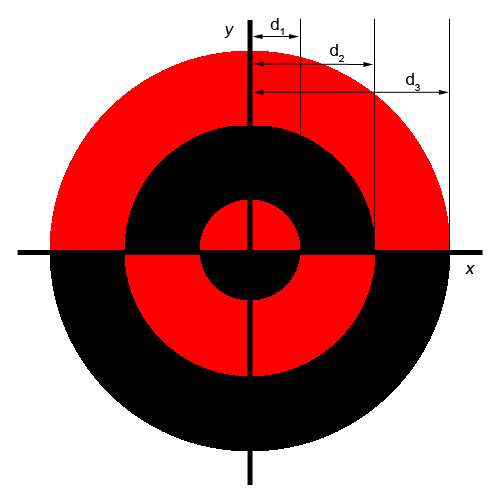
\includegraphics[width=0.5\textwidth]{img/concentric_circles}
  \caption{Concentric circles}
  \label{fig:concentric_circles}
\end{figure}

Although this problem can be approached with a multitude of classification techniques, we will compare the performance of the SVM with that of an EKF-trained MLP. The SVM is the more popular technique but it requires a lot of computational time. Consequently, the SVM is more appropriate for tasks with no time constraints rather than near real-time applications.

\section{Methodology}
\label{sec:methodology}

This section will explain the finer details involved in solving the concentric circle classification problem.

\subsection{Data Points}
\label{sec:data-points}

The random points were chosen from a uniform distribution within the shape as outlined in Equation~\eqref{eq:1}. Each point consisted of an x and y coordinate that was used as the input to the neural networks. Epochs of 200 points were generated with 100 points being from each class.

\begin{samepage}
\begin{alignat}{2}
  \label{eq:1}
  x &= \sqrt{r} \cos{\theta}, &\quad& 0 \leq r \leq d_3 \\
  y &= \sqrt{r} \sin{\theta}, && 0 \leq \theta < 2\pi \nonumber
\end{alignat}
\begin{gather}
  \text{where \(r\) and \(\theta\) are random variables from a uniform distribution} \nonumber
\end{gather}
\end{samepage}

\subsection{SVM}
\label{sec:svm-1}

The SVM classifier was trained using 200 epochs of data and its performance was observed during the training process. Inherently, the SVM algorithm is not an iterative algorithm, therefore training could only progress by retraining the algorithm with a larger training data set on each iteration. In order to generate a progressive measure of the error rate throughout the training process, the data from each new epoch was appended to all the previous epochs until all 200 epochs were being used as the training data. 

SVMs are relatively easy to use as there are not many parameters that need to be tuned. The radial basis function was used as the kernel function. In MATLAB, the SVM functions allow the user to specify the method used to find the hyperplane. Sequential minimal optimization was chosen as opposed to the traditional quadratic programming method simply because the former offered a significant speed increase. Different values of the C parameter (100, 500 and 2500) were also compared to determine their effect on processing time and respective classification performance of the SVM.

\subsection{EKF-trained MLP}
\label{sec:ekf-trained-mlp-1}

It quickly becomes apparent that the EKF-trained MLP is a much more complex algorithm for solving this classification problem. First, there are a number of parameters within the EKF that need to be adequately tuned to ensure that the algorithm does not become unstable. Second, the MLP network configuration can take a number of forms. These two reasons called for many simulations exploring the effects of all the different parameters. 

\subsubsection{Parameters}
\label{sec:parameters}

The discussion in \cite{Haykin2001} provides rough guidelines for setting parameters for EKF training algorithms. Our main concern is with the weight vector, desired output, error covariance matrix \(\left(\mathbf{P}\right)\), covariance matrix of the measurement noise \(\left(\mathbf{R}\right)\) and covariance matrix of the process noise \(\left(\mathbf{Q}\right)\).

\paragraph{Weight Vector}
There is no prior knowledge available about the weight vector and its effect on the performance of the MLP. The weight vector is initialized with random values between 0 and 1 from a uniform distribution.

\paragraph{Desired Output}
The standard desired output for neural networks is \(\pm1\). However, as explained in Section~\ref{sec:instabilities}, it was found through experience that a wider output range provided better classification results.

\paragraph{Error Covariance Matrix, \(\mathbf{P}\) }
The error covariance matrix, \(\mathbf{P}\), reflects the accuracy of weight vector estimate. Since the initial weight vector estimate is random, this reflects the lack of \textit{a priori} information and consequently there is a large error in this estimate. This can be represented by initializing \(\mathbf{P}\) to a large number. 

\paragraph{Covariance Matrix of the Measurement Noise, \(\mathbf{R}\) }
According to \cite{Haykin2001}, \(\mathbf{R}\) can be written as \(\mathbf{R}=\eta^{-1} \mathbf{I}\) where \(\eta\) represents the learning rate. The recommended range for \(\eta\) is \(0.001 - 1\).

\paragraph{Covariance Matrix of the Process Noise, \(\mathbf{Q}\) }
The covariance matrix of the process noise, \(\mathbf{Q} = q\mathbf{I}\), is an indication of how noisy the weight vector is at any instant in time. The recommended range for \(q\) is \(0-0.1\). Furthermore, \(\mathbf{Q}\) can be annealed to a lower limit on the order of \(10^{-6}\). In this case, annealing provides a way of limiting the noise in the process equation as training progresses. The idea is that as the algorithm undergoes more training epochs, the weight vector should be a much better estimate of the optimal state and therefore less noisy. 

\paragraph{Simulation Parameters}
In the end, the parameter values used in the simulations can be seen in Table~\ref{table:ekf_parameter_values}.

\begin{table}[ht]
  	\centering
  	\begin{tabular}{ l l }
		\rowcolor[gray]{0.8}
		\textbf{Parameter} & \textbf{Parameter Values} \\
  		\(\mathbf{P_0}\) & \( 10\mathbf{I}, 100\mathbf{I}, 1000\mathbf{I}, 10000\mathbf{I} \) \\
  		\(\mathbf{Q_0}\) & \( 0.1\mathbf{I}, 0.01\mathbf{I}, 0.001\mathbf{I} \) \\
 		\(\mathbf{R_0}\) & \( 1\mathbf{I}, 10\mathbf{I}, 100\mathbf{I}, 200\mathbf{I}, 500\mathbf{I}, 700\mathbf{I}, 900\mathbf{I} \) \\
  		Desired Output& \( \pm0.7, \pm1, \pm2, \pm5, \pm10 \) \\
  		Annealing& \( \text{true}, \text{false} \)
	\end{tabular}
	\caption{EKF Simulation Parameters}
	\label{table:ekf_parameter_values}
\end{table}

\subsubsection{MLP Network}
\label{sec:mlp-network}

In practice, the study of neural networks is highly problem dependent. As such, different MLP architectures were used to make relative comparisons with regards to their performance. A general form of the MLP architecture was shown in Figure~\ref{fig:mlp_network} and the networks used in the experiment follow this general form employing either 1 or 2 hidden layers. The different MLP configurations are listed in Table~\ref{table:network-configurations}.

\begin{table}[ht]
  \begin{center}
  \begin{tabular}[c]{>{\centering}m{0.2\textwidth} | >{\centering}m{0.2\textwidth} | >{\centering}m{0.2\textwidth}}
    \hline
    Number of Hidden Layers & Number of Hidden Nodes in First Layer & Number of Hidden Nodes in Second Layer \tabularnewline
    \hline \hline
    1 Layer & 10 & \tabularnewline
            & 20 & \tabularnewline
            & 30 & \tabularnewline
    \hline
    2 Layers & 4 & 3 \tabularnewline
             & 10 & 3 \tabularnewline
             & 20 & 6 \tabularnewline
             & 24 & 8 \tabularnewline
  \end{tabular}
  \end{center}
  \caption{MLP Network Configurations}
  \label{table:network-configurations}
\end{table}

All networks had 2 input nodes, one for the x coordinate and another for the y coordinate. Only one output node was necessary and the class was determined by the sign of the output - positive for red regions and negative for black regions. For networks with 2 hidden layers, the number of nodes in the second hidden layer was around \(\frac{1}{3}\) of the previous layer (according to the ``rule of thumb'' discussed in class). Biases were also included for each node within the network. The activation function used by each hidden node was the hyperbolic tangent function, \(\tanh\).

\section{Simulation Results}
\label{sec:simulation-results}

\subsection{SVM}
\label{sec:svm-2}

Overall the SVM algorithm performed very well. The results of the simulations can be seen in Figure~\ref{fig:svm-performance}. The decision boundaries produced by the SVMs with \(C=100, C=500, C=2500\) can be seen in Figures~\ref{fig:svm_classified_data_100}, \ref{fig:svm_classified_data_500} and \ref{fig:svm_classified_data_2500}, respectively. All three simulations attained error rates below \(1.5\%\). It is evident that best performance is achieved when \(C=2500\) which was able to achieve a classification rate of \(99.4\%\). According to \cite{Haykin2008}, a large value for C indicates that the SVM is more complex. In our case, this translates to better performance since the training data was of high quality. Thus, by trusting the training data, the SVM is more sensitive around boundaries between the two classes and provides better resolution.

\begin{figure}[!ht]
  \centering
  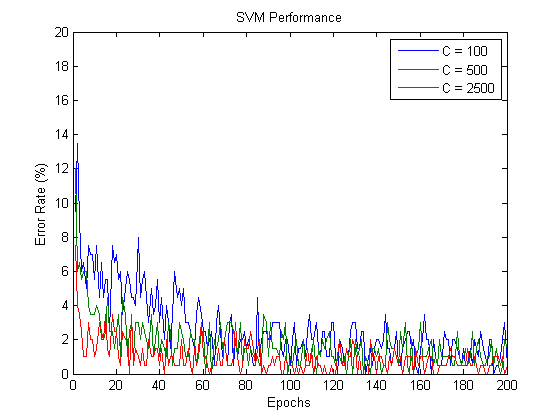
\includegraphics[width=0.6\textwidth]{img/svm_performance}
  \caption{SVM Performance}
  \label{fig:svm-performance}
\end{figure}

\begin{figure}[!ht]
  \centering
  \subfloat[Data classified by the SVM, C = 100, 98.5\% classification rate][Data classified by the SVM, C = 100, 98.5\% classification rate]{
    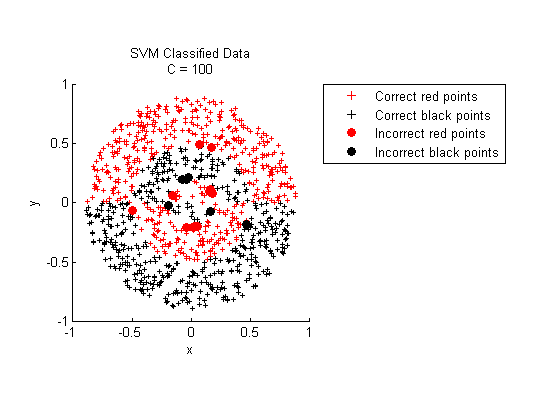
\includegraphics[width=0.5\textwidth]{img/svm_classified_data_c_100}
    \label{fig:svm_classified_data_100}
  }
  \qquad
  \subfloat[Data classified by the SVM, C = 500, 99.2\% classification rate][Data classified by the SVM, C = 500, 99.2\% classification rate]{
    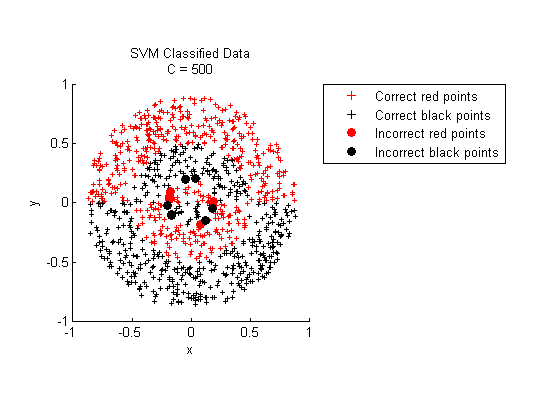
\includegraphics[width=0.5\textwidth]{img/svm_classified_data_c_500}
    \label{fig:svm_classified_data_500}
  }
  \qquad
  \subfloat[Data classified by the SVM, C = 2500, 99.4\% classification rate][Data classified by the SVM, C = 2500, 99.4\% classification rate]{
    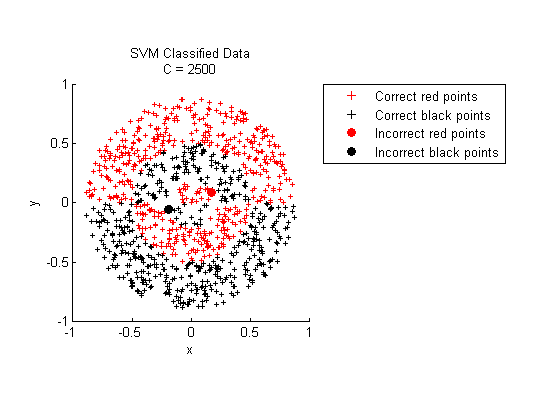
\includegraphics[width=0.5\textwidth]{img/svm_classified_data_c_2500}
    \label{fig:svm_classified_data_2500}
  }
  \caption{Data classified by the SVM}
  \label{fig:svm_classified_data}
\end{figure}
\clearpage

\subsection{EKF-trained MLP}
\label{sec:ekf-trained-mlp-2}

Overall, three batches of simulations were performed which will be referred to as Experiment 1, Experiment 2 and Experiment 3. 

\subsubsection{Experiment 1}
Experiment 1 used a desired output of \(\pm0.7\). Since this resulted in very poor results (further explained in Section~\ref{sec:effect-des-out-values}), the data has been omitted from the report. 

\subsubsection{Experiment 2}
Experiment 2 consisted of simulations employing every combination of the parameters shown in Table~\ref{table:ekf_parameters_exp_2}.

\begin{table}[ht]
  	\centering
  	\begin{tabular}{ l l }
		\rowcolor[gray]{0.8}
		\textbf{Parameter} & \textbf{Parameter Values} \\
		Network Configurations & 1 Layer: 10, 20, 30 nodes \\ 
		& 2 Layer: (4,3), (10,3), (20,6) nodes \\
  		\(\mathbf{P_0}\) & \( 100\mathbf{I} \) \\
  		\(\mathbf{Q_0}\) & \( 0.1\mathbf{I}, 0.01\mathbf{I}, 0.001\mathbf{I} \) \\
 		\(\mathbf{R_0}\) & \( 1\mathbf{I}, 10\mathbf{I}, 100\mathbf{I}, 200\mathbf{I}, 500\mathbf{I}\) \\
  		Desired Output& \( \pm1, \pm2, \pm5, \pm10 \) \\
  		Annealing& \( \text{true}, \text{false} \)
	\end{tabular}
	\caption{EKF Simulation Parameters for Experiment 2}
	\label{table:ekf_parameters_exp_2}
\end{table}

\paragraph{Instabilities}
\label{sec:instabilities}

Initially the greatest obstacle that was encountered was the instability of the training process. Two kinds of instabilities were encountered. One occurred when the EKF algorithm produced an error since an intermediate matrix within the algorithm was not positive definite. The second occurred when the performance of the algorithm became extremely unstable and at times oscillatory, as can be seen in Figure~\ref{fig:mlpekf_instability}.

\begin{figure}[H]
  \centering
  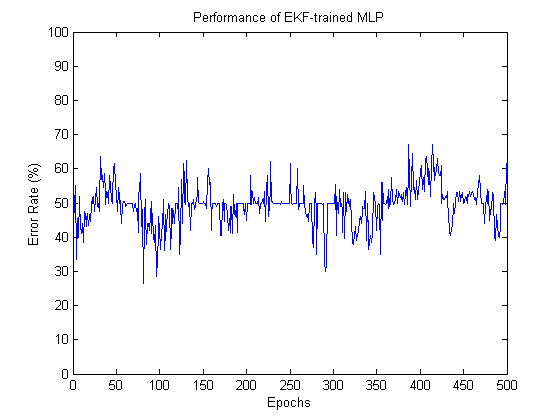
\includegraphics[width=0.6\textwidth]{img/mlpekf_instability}
  \caption{Example of unstable training process}
  \label{fig:mlpekf_instability}
\end{figure}


The first instability can be mostly attributed to low values of \(\mathbf{R_0}\) (i.e. \(\mathbf{R_0} < 500\mathbf{I}\)). Only the frequency of occurrence of the error was taken into account when making this observation. This instability is by no means exclusive to low values of \(\mathbf{R_0}\). Due to the fact that so many simulations, where \(\mathbf{R_0} < 500\mathbf{I}\), produced mathematical errors, they were not included in the analysis. Given the fact that these parameter values give rise to conditions that do not meet the positive definite requirement of the EKF, it is unreasonable to continue the analysis with these particular parameter values.

\paragraph{Performance of MLP Network Configurations}
\label{sec:mlp-netw-conf}

Data from the second batch of simulations was used to compare the performance of different MLP network configurations. As explained in Section~\ref{sec:instabilities} only data sets with \(\mathbf{R_0} = 500\mathbf{I}\) were used in this comparative analysis. Figure~\ref{fig:mlpekf_mlp_network_archs} shows the average performance of each network configuration over \(500\) training epochs.  

\begin{figure}[H]
  \centering
  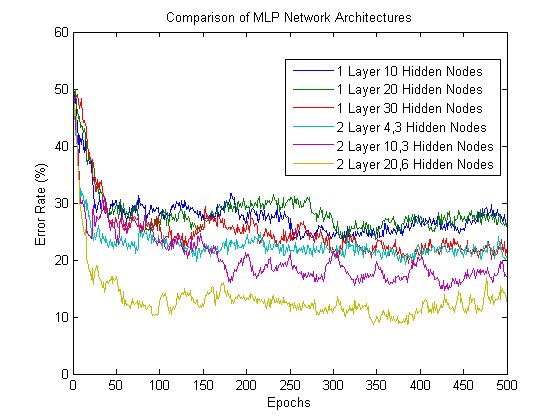
\includegraphics[width=0.6\textwidth]{img/mlpekf_mlp_network_archs}
  \caption{Comparison of various MLP Network Configurations}
  \label{fig:mlpekf_mlp_network_archs}
\end{figure}

These results clearly indicate that on average the more complex the network, the better the performance. Furthermore, it's interesting to see that a network with a single hidden layer does not gain a significant performance increase with an increased number of hidden nodes. On the other hand, increasing the number of hidden nodes in a network with two hidden layers, delivers much greater performance gains. Although it cannot be seen from these averaged results, the more complex networks also exhibited smoother and more stable performance during the training process. A possible interpretation of this result is that more complex networks are less reliant on the values of initial parameters for stability.

\paragraph{Effect of Desired Output Values}
\label{sec:effect-des-out-values}

Throughout this experiment it was noted that different values for the desired output had profound effects on the stability of the algorithm's performance during the training process. It was suggested in class that the desired output value be set to \(\pm 0.7\), since the activation function, \(\tanh\), had an output range of \(\pm 1\). This turned out to be extremely detrimental to the algorithm's performance. The performance during the training process was extremely unstable. The simplest explanation for this effect is the fact that the output of the network is not necessarily limited to the range of the activation function and it depends on the architecture. Furthermore, if the range of the desired output is small the algorithm can have a difficult time fitting an optimal decision surface that will be able to differentiate between the very tight boundaries. This agrees with the results of simulations that had wider ranges for the desired output. \textit{The larger the range the more stable the performance during the training process.} Figure~\ref{fig:mlpekf_desired_output_values} compares the performance while using various values for the desired output.

\begin{figure}[!ht]
  \centering
  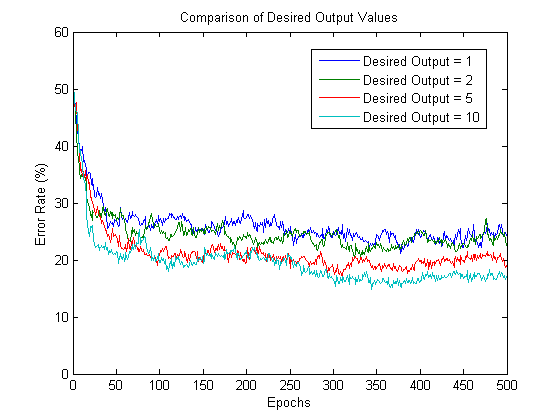
\includegraphics[width=0.6\textwidth]{img/mlpekf_desired_output_values}
  \caption{Performance comparison of various desired output values}
  \label{fig:mlpekf_desired_output_values}
\end{figure}

\subsubsection{Experiment 3}
Experiment 3 explored the parameters in Table~\ref{table:ekf_parameters_exp_3}. Experiment 3 was motivated by the knowledge gained with the results from Experiment 2:
\begin{itemize}
\item Increasing the complexity of the network, increases performance
\item Larger desired output values ensured more stability during the training process
\item Would larger initial values of the covariance matrix of the measurement noise \(\left(\mathbf{R_0}\right)\) improve performance and stability?
\item How does the error covariance matrix \(\left(\mathbf{P_0}\right)\) and the covariance matrix of the process noise \(\left(\mathbf{Q_0}\right)\) affect performance and stability?
\end{itemize}
Furthermore, by limiting the experiment to one network configuration, a better comparison could be made of the other parameters.

\begin{table}[ht]
  	\centering
  	\begin{tabular}{ l l }
		\rowcolor[gray]{0.8}
		\textbf{Parameter} & \textbf{Parameter Values} \\
		Network Configurations & 2 Layer: (24,8) nodes \\
  		\(\mathbf{P_0}\) & \( 10\mathbf{I}, 100\mathbf{I}, 1000\mathbf{I}, 10000\mathbf{I} \) \\
  		\(\mathbf{Q_0}\) & \( 0.1\mathbf{I}, 0.01\mathbf{I}, 0.001\mathbf{I} \) \\
 		\(\mathbf{R_0}\) & \( 10\mathbf{I}, 100\mathbf{I}, 200\mathbf{I}, 500\mathbf{I}, 700\mathbf{I}, 900\mathbf{I}\) \\
  		Desired Output& \( \pm10 \) \\
  		Annealing& \( \text{true}, \text{false} \)
	\end{tabular}
	\caption{EKF Simulation Parameters for Experiment 3}
	\label{table:ekf_parameters_exp_3}
\end{table}

It should be noted that the analysis for Experiment 3 also uses data sets where \(\mathbf{R_0} \geq 500\mathbf{I}\) because of the unstable results.

\paragraph{Initial Error Covariance Matrix, \(\mathbf{P_0}\)}
\label{sec:p_0}

Figure~\ref{fig:mlpekf_compare_p} compares the averaged performance of the simulations for different values of \(\mathbf{P_0}\). A trend emerges where decreasing values of \(\mathbf{P_0}\) offer better performance, with \(\mathbf{P_0}=10\mathbf{I}\) slightly outperforming \(\mathbf{P_0}=100\mathbf{I}\). This indicates that the initial estimate of the state may not be that far off the optimal state. Furthermore, it could be stated that larger values of \(\mathbf{P_0}\) simply require more training epochs to reach a better estimate of the state. 

Since \(\mathbf{P_0}=10000\mathbf{I}\) showed poor performance over \(500\) training epochs, these data sets were removed from the rest of the analysis.

\begin{figure}[H]
  \centering
  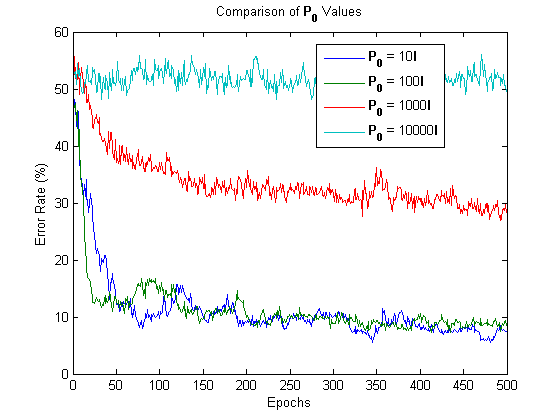
\includegraphics[width=0.6\textwidth]{img/mlpekf_compare_p}
  \caption{Comparison of different values for \(\mathbf{P_0}\)}
  \label{fig:mlpekf_compare_p}
\end{figure}

\paragraph{Initial Measurement Noise Covariance Matrix, \(\mathbf{R_0}\)}
\label{sec:r_0}

As was noticed in Experiment 2, simulations where \(\mathbf{R_0} < 500\mathbf{I}\) produce unstable results. However, by exploring larger values of \(\mathbf{R_0}\), we can conclude that larger values do increase performance as shown in Figure~\ref{fig:mlpekf_compare_r_no_p10000}.

\begin{figure}[H]
  \centering
  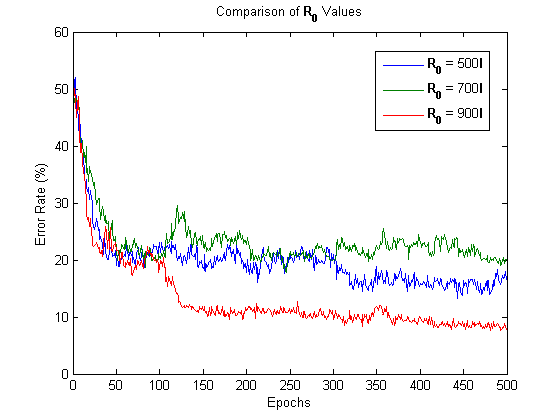
\includegraphics[width=0.6\textwidth]{img/mlpekf_compare_r_no_p10000}
  \caption{Comparison of different values for \(\mathbf{R_0}\)}
  \label{fig:mlpekf_compare_r_no_p10000}
\end{figure}

\paragraph{Initial Process Noise Covariance Matrix, \(\mathbf{Q_0}\)}
\label{sec:q_0}

From Figure~\ref{fig:mlpekf_compare_q_no_p10000}, we observe that performance increases as \(\mathbf{Q_0}\) decreases. A possible explanation of this trend is that a smaller value of \(\mathbf{Q_0}\) limits the degree of allowable change in the weight vector components, thus making the algorithm less susceptible to reach suboptimal weight vector variations.

\begin{figure}[H]
  \centering
  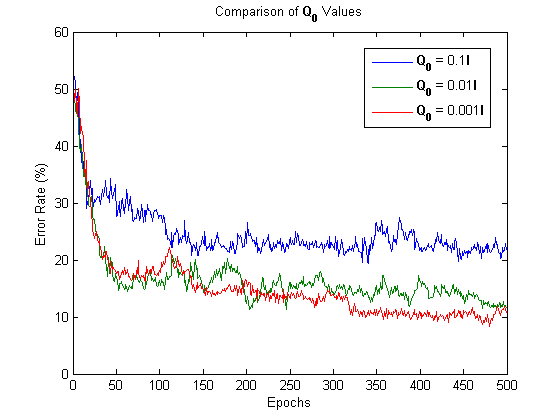
\includegraphics[width=0.6\textwidth]{img/mlpekf_compare_q_no_p10000}
  \caption{Comparison of different values for \(\mathbf{Q_0}\)}
  \label{fig:mlpekf_compare_q_no_p10000}
\end{figure}

As was suggested in \cite{Haykin2001}, annealing could be applied to \(\mathbf{Q_0}\). The results are presented in Figure~\ref{fig:annealing_effects}. The results are surprising in that annealing should help with faster convergence and avoid divergence at the end of training process. Only Figure~\ref{fig:mlpekf_annealing_effects_q_001} shows a slightly faster convergence with annealing. In addition, Figure~\ref{fig:mlpekf_annealing_effects} shows that annealing appears to hinder performance.

\begin{figure}[H]
	\centering
  	\subfloat[Overall Effects of Annealing \(\mathbf{Q_0}\)][Overall Effects of Annealing \(\mathbf{Q_0}\)]{
  		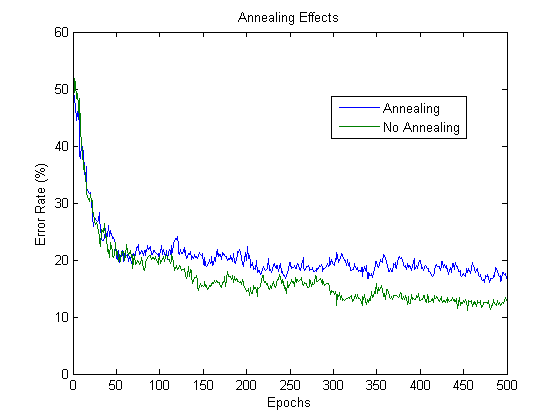
\includegraphics[width=0.45\textwidth]{img/mlpekf_annealing_effects}
		\label{fig:mlpekf_annealing_effects}
  	}
  	\qquad
	\subfloat[Effects of Annealing \(\mathbf{Q_0} = 0.1\)][Effects of Annealing \(\mathbf{Q_0} = 0.1\)]{
  		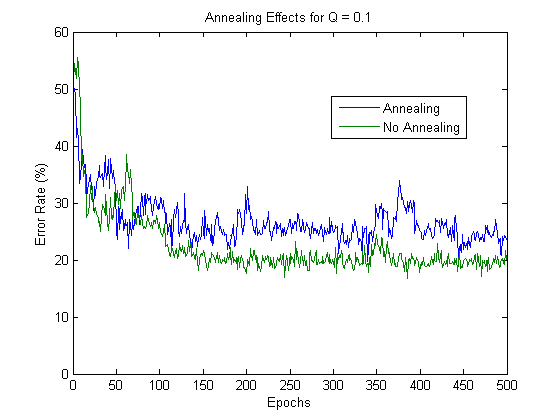
\includegraphics[width=0.45\textwidth]{img/mlpekf_annealing_effects_q_01}
	  	\label{fig:mlpekf_annealing_effects_q_01}
  	}
  	\qquad
  	\subfloat[Effects of Annealing \(\mathbf{Q_0} = 0.01\)][Effects of Annealing \(\mathbf{Q_0} = 0.01\)]{
  		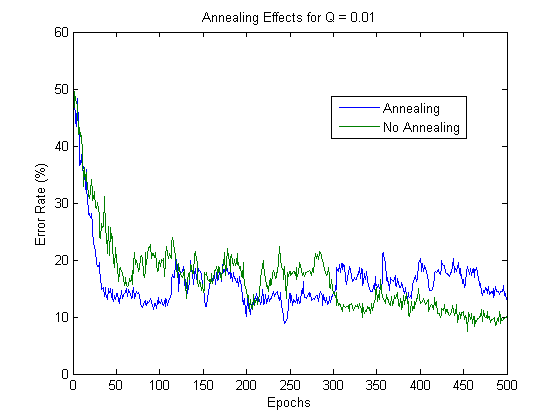
\includegraphics[width=0.45\textwidth]{img/mlpekf_annealing_effects_q_001}
	  	\label{fig:mlpekf_annealing_effects_q_001}
  	}
  	\qquad
  	\subfloat[Effects of Annealing \(\mathbf{Q_0} = 0.001\)][Effects of Annealing \(\mathbf{Q_0} = 0.001\)]{
  		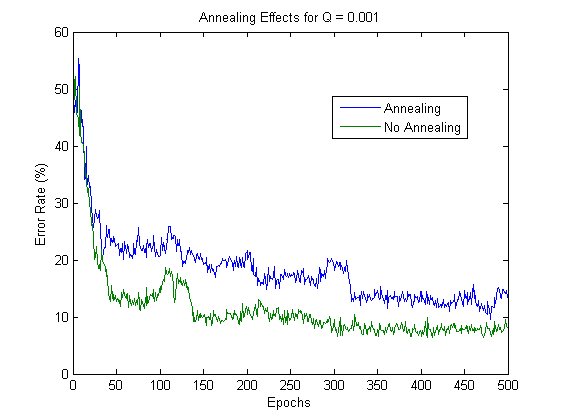
\includegraphics[width=0.45\textwidth]{img/mlpekf_annealing_effects_q_0001}
	  	\label{fig:mlpekf_annealing_effects_q_0001}
  	}
	\caption{Effects of Annealing}
	\label{fig:annealing_effects}
\end{figure}

\paragraph{Optimal Parameters}

As a result of this experiment, the best parameters for this network configuration are \(\mathbf{Q_0} = 0.001\), \(\mathbf{R_0} = 900\), \(\mathbf{P_0} = 10\), desired output = \(10\) and no annealing. Figure~\ref{fig:mlpekf_best_perf} shows the performance of the MLP trained using these parameters. It reaches a classification rate of 95\% within 30 epochs and averages approximately 96\% for the remainder of the training epochs.

\begin{figure}[H]
  \centering
  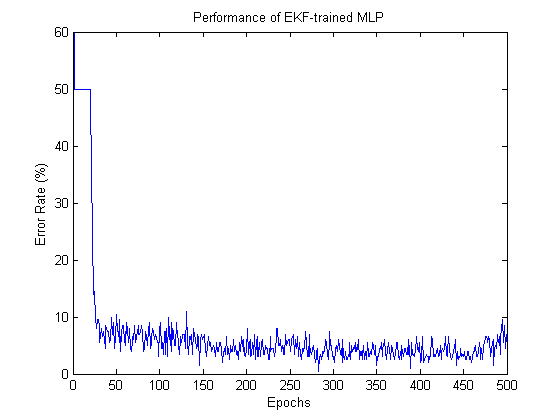
\includegraphics[width=0.6\textwidth]{img/mlpekf_best_perf}
  \caption{Performance of MLP trained using the best parameters for the EKF algorithm}
  \label{fig:mlpekf_best_perf}
\end{figure}

\section{Conclusion}
In conclusion, both algorithms resulted in amazing classification performance. The SVM achieved a classification rate of 99.4\% whereas the EKF-trained MLP network achieved approximately 96\%. Both of these results exceeded the expectation of around 75\% that was mentioned in class. Although the SVM proved to be more accurate, it's network was much more complex than the 2 layer MLP network with a total of 32 hidden nodes. The SVM required the use of over 3000 support vectors.

In many situations computational time can be of great concern. For a data set of 200 data points and 200 epochs, the computational time required by the SVM was 10 minutes and 2 minutes for the EKF-trained MLP. This is a significant difference. It is further exacerbated by the fact that the EKF is an iterative algorithm. Thus, if new data becomes available only the new data needs to be presented to the EKF. The SVM, on the other hand, would need to be completely retrained using the entire data set.

Overall, the SVM offers great accuracy at the cost of computational resources, namely memory and time. The EKF-trained MLP provides a short training phase, a lightweight network as well as comparable classification performance to that of the SVM. In the end, application of either of these algorithms will always be problem dependent.

\clearpage

\appendix
\section{MATLAB Code}
The MATLAB code is available upon request.

\clearpage

% References
\bibliographystyle{IEEEtran}
%\bibliography{IEEEabrv,TMS,Thesis}
\bibliography{/cygdrive/c/Users/Phil/Documents/School/References/Machine_Learning}

\end{document}